%
% teil1.tex -- Beispiel-File für das Paper
%
% (c) 2020 Prof Dr Andreas Müller, Hochschule Rapperswil
%
% !TEX root = ../../buch.tex
% !TEX encoding = UTF-8
%
\section{Lineares Medium\label{particles:section:linear}}
\kopfrechts{Lineares Medium}
% TODO: Quellenangaben
% [ ]: https://en.wikipedia.org/wiki/Linearity
% [ ]: Lineare Algebra: Eine anwendungsorientierte Einführung, Seite: 27, ISBN: 978-3-662-67865-7, Published: 01 September 2023, DOI: https://doi.org/10.1007/978-3-662-67866-4

\subsection{Was ist Linearität?}
Für den einfachsten und üblichsten Fall nimmt man oft ein \emph{lineares Medium} an.
Solch ein Medium nennt man \emph{linear}, wenn dessen Definition sowohl \emph{additiv}
\[
    f(x_{1} + y_{1}, \ldots, x_{n} + y_{n}) 
    = 
    f(x_{1}, \ldots, x_{n}) 
    + 
    f(y_{1}, \ldots, y_{n}),
\]
als auch \emph{homogen}
\[
    f(\lambda x_{1}, \ldots, \lambda x_{n}) 
    = 
    \lambda f(x_{1}, \ldots, x_{n})
\]
ist.
Hierbei ist angemerkt, dass $x_{k}$, $y_{k}$ und $\lambda$ nicht rein reell sein müssen, 
sondern einem beliebigen Vektorraum angehören können, was für den zweidimensionalen Fall wichtig ist.

In der Wellentheorie bedeutet dies, 
dass die Materialeigenschaften -- beispielsweise die Elastizität -- nicht von der Amplitude der Welle abhängen.
Diese Elastizität eines Mediums lässt sich durch das \emph{hookesche Gesetz}
\[
    \Delta l
    = 
    \frac{F}{D}
    \quad
    \left(D = \text{const.} 
    \Rightarrow 
    \frac{\partial D}{\partial F} 
    \overset{!}{=} 
    0 
    \quad 
    \forall F \right)
    \label{particles:eq:hookesches-gesetz},
\]
welches bereits in abschnitt \mytodo{Verweis Elastizitätstheorie} verwendet wurde, beschreiben.
Dabei beschreibt $\Delta l$ die Distanzänderung zweier Punkte,
$F$ die dazwischen wirkende Kraft und $D$ einen Proportionalitätsfaktor.
Mittels Substitution kann man nun darauf schliessen, 
dass es sich hierbei tatsächlich um eine lineare Funktion handeln muss.

\begin{figure}
    \centering
    \subfigure[]{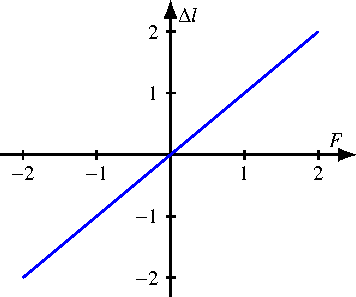
\includegraphics{./papers/particles/figures/out/lineares_medium_deformation.pdf}\label{particles:fig:lin-medium:deform}}\hfill
    \subfigure[]{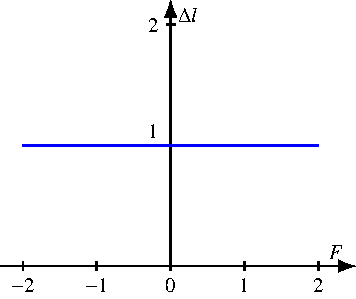
\includegraphics{./papers/particles/figures/out/lineares_medium_elast_modul.pdf}\label{particles:fig:lin-medium:elast-modul}}
    \caption{Deformation~(a) und Elastisches Modul~(b) eines linearen Mediums mit konstantem Faktor $D = 1$.}
\end{figure}

\subsection{Superpositionsprinzip}\label{particles:section:lin-medium:superposition} % TODO: Subsection umschreiben
Das Superpositionsprinzip fasst die Bedingungen zur Linearität nochmal etwas schöner in eine Formel zusammen, 
nämlich
\[
    T(\lambda x + \mu y)
    = 
    \lambda T(x) 
    + 
    \mu T(y).
\]
Blickt man wieder auf die Wellentheorie, so bedeutet dies, dass sich Wellen in linearen Medien überlagern, sich aber nicht gegenseitig beeinflussen.
Dies kann man schön anhand zweier sich kreuzende Laserstrahlen im Vakuum veranschaulichen, wie sie in Abbildung \mytodo{Abbildung zweier Laserstrahlen, die sich kreuzen, lokal interferieren, jedoch den weiteren Verlauf nicht verändern.} gezeigt werden.
Lokal interferieren diese Laserstrahlen zwar, stören jedoch nicht ihren weiteren Verlauf.


\subsection{Wellengleichung}\label{particles:section:lin-medium:wellengleichung}
Die Wellengleichung 
\[
    \frac{\d^2 u}{\d t^2} = c^2 \cdot \nabla^2 u, \label{particles:eq:wellengleichung}
\]
hat in vielen Feldern anwendung.
Dabei steht auf der linken Seite die zweite Ableitung nach der Zeit und auf der rechten die räumliche Ableitung sowie die Konstante $c^2$.
Eine massgebende Anname ist dabei die Linearität des Mediums.
Dies wird ersichtlicher, wenn man die Herleitung der Wellengleichung aus zum Beispiel den Maxwell-Gleicungen betrachtet.

\subsubsection{Herleitung}
Zur Herleitung der Wellengleichung im Elektrischen Feld ist die Identität
\[
    \nabla \times \nabla \times \mathbf{U} = \nabla(\nabla \cdot \mathbf{U}) - \nabla^2 \mathbf{U}\label{particles:eq:curl-identity}
\]
notwendig. 
Diese wurde in Abschnit \mytodo{Wurde diese schon vorgestellt?} bereits hergeleitet und gilt für sämmtliche Vektorfelder.

Als erster Schritt der Herleitung wird $\rho = 0$, also ein Medium ohne freie Ladungsträger, angenommen.
Das gausssche Gesetz
\[
    \nabla \cdot \mathbf{D} = \rho_\text{frei}
\]
wird unter dieser Annahme zu
\[
    \nabla \cdot \mathbf{D} = 0.\label{particles:eq:gauss}
\]
Weiter wird der Erweiterte Durchflutungssatz
\[
    \nabla \times \mathbf{H} = \mathbf{j}_\text{frei} + \frac{\d \mathbf{D}}{dt}
\]
durch Annahme einer Stromdichte von $\mathbf{j}_\text{frei} = 0$ zu
\[
    \nabla \times \mathbf{H} = \frac{\d \mathbf{D}}{dt}.\label{particles:eq:durchflutungssatz}
\]
Das Induktionsgesetz
\[
    \nabla \times \mathbf{E} = -\frac{\d \mathbf{B}}{\d t}\label{particles:eq:induktionsgesetz}
\]
wird ebenfalls benötigt.

Um die elektrische Flussdichte $\mathbf{D}$ mit dem elektrischen Feld $\mathbf{E}$ in Relation zu bringen, wird die Permittivität $\varepsilon$ beigezogen.
Die Permittivität ist abhängig vom Medium. 
$\mathbf{D}$ und $\mathbf{E}$ stehen also im Verhältnis
\[
    \mathbf{D} = \varepsilon \mathbf{E}.
\]
Ein ähnliches Verhältnis stellt sich zwischen der magnetischen Flussdichte $\mathbf{B}$ und der magnetischen Feldstärke $\mathbf{H}$ ein, wobei das Verhältnis durch die Permeabilität $\mu$ als
\[
    \mathbf{B} = \mu \mathbf{H} \quad \text{bzw.} \quad \mathbf{H} = \frac{\mathbf{B}}{\mu}
\]
gegeben wird.
Auch die Permeabilität ist mediumabhängig.

Zunächst wird das Induktionsgesetz~\ref{particles:eq:induktionsgesetz} durch den curl zu
\begin{align}
    \nabla \times \nabla \times \mathbf{E} 
        &= - \nabla \times \frac{\d\mathbf{B}}{\d t} \\
        &= - \frac{\d}{\d t} \nabla \times \mathbf{B}
\end{align}
erweitert.
Durch die Identität~\ref{particles:eq:curl-identity} und der Permeabilität kann das Resultat zu
\[
    \nabla(\nabla \cdot \mathbf{E}) - \nabla^2 \mathbf{E} = -\mu \frac{\d}{\d t} \nabla \times \mathbf{H}
\]
ungeformt werden.
Durch Einsetzen des gaussschen Gesetz~\ref{particles:eq:gauss} und dem Durchflutungssatz~\ref{particles:eq:durchflutungssatz} entsteht
\[
    - \nabla^2 \mathbf{E} = -\mu \frac{\d}{\d t} \frac{\d \mathbf{D}}{\d t},
\]
und schliesslich entsteht mit $\mathbf{D} = \varepsilon \mathbf{E}$
\[
    \nabla^2 \mathbf{E} = \mu\varepsilon \frac{\d^2 \mathbf{E}}{\d t^2} 
    \quad \text{bzw.} \quad
    \frac{\d^2 \mathbf{E}}{\d t^2} = \frac{1}{\mu \varepsilon} \nabla^2 \mathbf{E},
\]
was der Wellengleichung entspricht.
Durch ähnliches Vorgehen kann diese auch für die magnetische Feldstärke $\mathbf{B}$ hergeleitet werden.

Dabei wird durch Parametervergleich mit der Wellengleichung aus~\ref{particles:eq:wellengleichung} klar, dass die Ausbreitungsgeschwindigkeit
\[
    c = \frac{1}{\sqrt{\mu\varepsilon}}\label{particles:eq:lichtgeschwindigkeit}
\]
beträgt.


\subsection{Schwinger-Limit}\label{particles:section:lin-medium:schwinger}
Bei extrem hohen Feldstärken tritt ein Phänomen auf, wobei das Vakuum selbst nichtlinear wird.
Dieser Übergang zur Nichtlinearität des Vakuums nennt man das \emph{Schwinger-Limit}\mytodo{Quellenangabe}, benannt nach Julian Schwinger, welcher 1951 dieses Phänomen erstmals theoretisierte.
Da es sich hierbei um elektrische und magnetische Feldstärken im Bereich von $10^{18}\,\frac{\text{V}}{\text{m}}$ und $10^9\,\text{T}$ handelt, konnte dieses Limit bisher noch nicht konkret nachgewiesen oder gemessen werden.
Es ist entsprechend noch immer Bestandteil aktueller Forschungen. \mytodo{Quelle hierfür angeben}

Beschränkt man sich jedoch nicht nur auf das Vakuum, so findet man Medien, welche bereits bei deutlich kleineren Feldstärken nichtlineare Eigenschaften aufweisen.
Ein Beispiel von solchen nichtlinearen Werkstoffen sind, wie~\ref{particles:frequenzverdopplung} demonstriert, Kristalle zur Frequenzverdoppelung.
Diese werden zum Beispiel in grünen Laserpointern eingesetzt, was die Verwendung von preiswerteren Infrarot-Laserdioden anstelle der teureren grünen Ausführung erlaubt.
